\documentclass{standalone}
\usepackage{tikz}
\usetikzlibrary{patterns, positioning}


\begin{document}
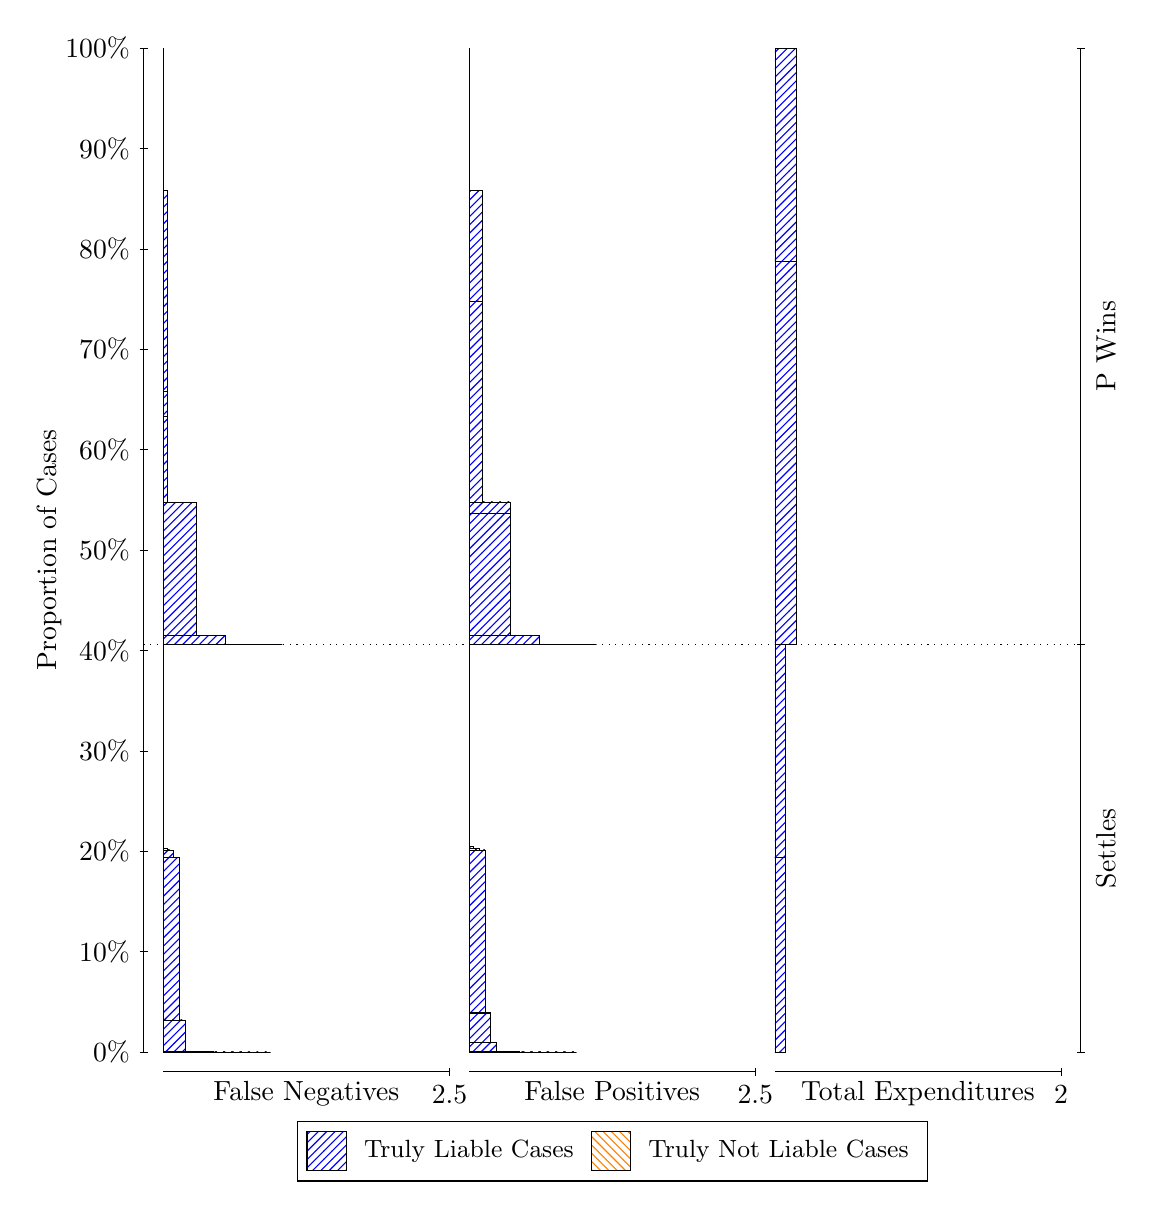
\begin{tikzpicture}
\draw[black, very thin] (1.5,1.75) -- (1.5,14.5);
\node[rotate=90, text=black, anchor=center] at (0.3, 8.125) {Proportion of Cases};
\draw[black, very thin] (1.45,1.75) -- (1.55,1.75);
\node[text=black, anchor=east] at (1.45, 1.75) {0\%};
\draw[black, very thin] (1.45,3.025) -- (1.55,3.025);
\node[text=black, anchor=east] at (1.45, 3.025) {10\%};
\draw[black, very thin] (1.45,4.3) -- (1.55,4.3);
\node[text=black, anchor=east] at (1.45, 4.3) {20\%};
\draw[black, very thin] (1.45,5.575) -- (1.55,5.575);
\node[text=black, anchor=east] at (1.45, 5.575) {30\%};
\draw[black, very thin] (1.45,6.85) -- (1.55,6.85);
\node[text=black, anchor=east] at (1.45, 6.85) {40\%};
\draw[black, very thin] (1.45,8.125) -- (1.55,8.125);
\node[text=black, anchor=east] at (1.45, 8.125) {50\%};
\draw[black, very thin] (1.45,9.4) -- (1.55,9.4);
\node[text=black, anchor=east] at (1.45, 9.4) {60\%};
\draw[black, very thin] (1.45,10.675) -- (1.55,10.675);
\node[text=black, anchor=east] at (1.45, 10.675) {70\%};
\draw[black, very thin] (1.45,11.95) -- (1.55,11.95);
\node[text=black, anchor=east] at (1.45, 11.95) {80\%};
\draw[black, very thin] (1.45,13.225) -- (1.55,13.225);
\node[text=black, anchor=east] at (1.45, 13.225) {90\%};
\draw[black, very thin] (1.45,14.5) -- (1.55,14.5);
\node[text=black, anchor=east] at (1.45, 14.5) {100\%};

\draw[black, very thin] (13.4,1.75) -- (13.4,14.5);
\draw[black, very thin] (13.35,1.75) -- (13.45,1.75);
\node[anchor=west] at (13.35, 1.75) {};
\draw[black, very thin] (13.35,6.9269) -- (13.45,6.9269);
\node[anchor=west] at (13.35, 6.9269) {};
\draw[black, very thin] (13.35,14.5) -- (13.45,14.5);
\node[anchor=west] at (13.35, 14.5) {};

\draw[black, very thin, pattern color=blue, pattern=north east lines] (1.75,1.75) rectangle (3.1125,1.75);
\draw[black, very thin, pattern color=blue, pattern=north east lines] (1.75,1.75) rectangle (2.8218,1.75);
\draw[black, very thin, pattern color=blue, pattern=north east lines] (1.75,1.75) rectangle (2.7492,1.75);
\draw[black, very thin, pattern color=blue, pattern=north east lines] (1.75,1.75) rectangle (2.6765,1.75);
\draw[black, very thin, pattern color=blue, pattern=north east lines] (1.75,1.75) rectangle (2.5312,1.75);
\draw[black, very thin, pattern color=blue, pattern=north east lines] (1.75,1.75) rectangle (2.4585,1.75);
\draw[black, very thin, pattern color=blue, pattern=north east lines] (1.75,1.75) rectangle (2.3858,1.7531);
\draw[black, very thin, pattern color=blue, pattern=north east lines] (1.75,1.7531) rectangle (2.3132,1.7531);
\draw[black, very thin, pattern color=blue, pattern=north east lines] (1.75,1.7531) rectangle (2.2405,1.7533);
\draw[black, very thin, pattern color=blue, pattern=north east lines] (1.75,1.7533) rectangle (2.1678,1.7541);
\draw[black, very thin, pattern color=blue, pattern=north east lines] (1.75,1.7541) rectangle (2.0952,1.7543);
\draw[black, very thin, pattern color=blue, pattern=north east lines] (1.75,1.7543) rectangle (2.0952,1.7554);
\draw[black, very thin, pattern color=blue, pattern=north east lines] (1.75,1.7554) rectangle (2.0225,2.1567);
\draw[black, very thin, pattern color=blue, pattern=north east lines] (1.75,2.1567) rectangle (1.9498,2.1569);
\draw[black, very thin, pattern color=blue, pattern=north east lines] (1.75,2.1569) rectangle (1.9498,4.2249);
\draw[black, very thin, pattern color=blue, pattern=north east lines] (1.75,4.2249) rectangle (1.8772,4.3174);
\draw[black, very thin, pattern color=blue, pattern=north east lines] (1.75,4.3174) rectangle (1.8045,4.3384);
\draw[black, very thin, pattern color=orange, pattern=north west lines] (1.75,4.3384) rectangle (1.75,4.3384);
\draw[black, very thin, pattern color=blue, pattern=north east lines] (1.75,4.3384) rectangle (1.75,6.9269);
\draw[black, very thin, pattern color=blue, pattern=north east lines] (1.75,6.9269) rectangle (3.2578,6.9269);
\draw[black, very thin, pattern color=blue, pattern=north east lines] (1.75,6.9269) rectangle (2.8945,6.9281);
\draw[black, very thin, pattern color=blue, pattern=north east lines] (1.75,6.9281) rectangle (2.5312,7.0432);
\draw[black, very thin, pattern color=blue, pattern=north east lines] (1.75,7.0432) rectangle (2.1678,8.7329);
\draw[black, very thin, pattern color=blue, pattern=north east lines] (1.75,8.7329) rectangle (1.8045,9.8202);
\draw[black, very thin, pattern color=blue, pattern=north east lines] (1.75,9.8202) rectangle (1.8045,10.139);
\draw[black, very thin, pattern color=blue, pattern=north east lines] (1.75,10.139) rectangle (1.8045,12.692);
\draw[black, very thin, pattern color=orange, pattern=north west lines] (1.75,12.692) rectangle (1.75,12.692);
\draw[black, very thin, pattern color=blue, pattern=north east lines] (1.75,12.692) rectangle (1.75,14.5);
\draw[black, very thin, pattern color=orange, pattern=north west lines] (5.6333,1.75) rectangle (6.9958,1.75);
\draw[black, very thin, pattern color=blue, pattern=north east lines] (5.6333,1.75) rectangle (6.9958,1.75);
\draw[black, very thin, pattern color=orange, pattern=north west lines] (5.6333,1.75) rectangle (6.8505,1.75);
\draw[black, very thin, pattern color=blue, pattern=north east lines] (5.6333,1.75) rectangle (6.8505,1.75);
\draw[black, very thin, pattern color=orange, pattern=north west lines] (5.6333,1.75) rectangle (6.7052,1.75);
\draw[black, very thin, pattern color=blue, pattern=north east lines] (5.6333,1.75) rectangle (6.7052,1.75);
\draw[black, very thin, pattern color=blue, pattern=north east lines] (5.6333,1.75) rectangle (6.6325,1.75);
\draw[black, very thin, pattern color=blue, pattern=north east lines] (5.6333,1.75) rectangle (6.4872,1.75);
\draw[black, very thin, pattern color=orange, pattern=north west lines] (5.6333,1.75) rectangle (6.4145,1.75);
\draw[black, very thin, pattern color=blue, pattern=north east lines] (5.6333,1.75) rectangle (6.4145,1.75);
\draw[black, very thin, pattern color=blue, pattern=north east lines] (5.6333,1.75) rectangle (6.3418,1.751);
\draw[black, very thin, pattern color=blue, pattern=north east lines] (5.6333,1.751) rectangle (6.2692,1.7533);
\draw[black, very thin, pattern color=orange, pattern=north west lines] (5.6333,1.7533) rectangle (6.2692,1.7533);
\draw[black, very thin, pattern color=blue, pattern=north east lines] (5.6333,1.7533) rectangle (6.2692,1.7533);
\draw[black, very thin, pattern color=blue, pattern=north east lines] (5.6333,1.7533) rectangle (6.1238,1.7542);
\draw[black, very thin, pattern color=orange, pattern=north west lines] (5.6333,1.7542) rectangle (6.1238,1.7542);
\draw[black, very thin, pattern color=blue, pattern=north east lines] (5.6333,1.7542) rectangle (6.1238,1.7542);
\draw[black, very thin, pattern color=blue, pattern=north east lines] (5.6333,1.7542) rectangle (6.0512,1.755);
\draw[black, very thin, pattern color=blue, pattern=north east lines] (5.6333,1.755) rectangle (5.9785,1.8675);
\draw[black, very thin, pattern color=blue, pattern=north east lines] (5.6333,1.8675) rectangle (5.9058,2.2477);
\draw[black, very thin, pattern color=blue, pattern=north east lines] (5.6333,2.2477) rectangle (5.9058,2.2479);
\draw[black, very thin, pattern color=orange, pattern=north west lines] (5.6333,2.2479) rectangle (5.8332,2.2479);
\draw[black, very thin, pattern color=blue, pattern=north east lines] (5.6333,2.2479) rectangle (5.8332,4.3171);
\draw[black, very thin, pattern color=blue, pattern=north east lines] (5.6333,4.3171) rectangle (5.7605,4.3383);
\draw[black, very thin, pattern color=blue, pattern=north east lines] (5.6333,4.3383) rectangle (5.7605,4.3385);
\draw[black, very thin, pattern color=blue, pattern=north east lines] (5.6333,4.3385) rectangle (5.6878,4.3596);
\draw[black, very thin, pattern color=blue, pattern=north east lines] (5.6333,4.3596) rectangle (5.6333,6.9269);
\draw[black, very thin, pattern color=orange, pattern=north west lines] (5.6333,6.9269) rectangle (7.2502,6.9269);
\draw[black, very thin, pattern color=blue, pattern=north east lines] (5.6333,6.9269) rectangle (7.2502,6.9269);
\draw[black, very thin, pattern color=orange, pattern=north west lines] (5.6333,6.9269) rectangle (6.8868,6.9269);
\draw[black, very thin, pattern color=blue, pattern=north east lines] (5.6333,6.9269) rectangle (6.8868,6.9281);
\draw[black, very thin, pattern color=orange, pattern=north west lines] (5.6333,6.9281) rectangle (6.5235,6.9281);
\draw[black, very thin, pattern color=blue, pattern=north east lines] (5.6333,6.9281) rectangle (6.5235,7.0454);
\draw[black, very thin, pattern color=blue, pattern=north east lines] (5.6333,7.0454) rectangle (6.1602,8.5873);
\draw[black, very thin, pattern color=orange, pattern=north west lines] (5.6333,8.5873) rectangle (6.1602,8.5873);
\draw[black, very thin, pattern color=blue, pattern=north east lines] (5.6333,8.5873) rectangle (6.1602,8.7351);
\draw[black, very thin, pattern color=blue, pattern=north east lines] (5.6333,8.7351) rectangle (5.7968,11.288);
\draw[black, very thin, pattern color=orange, pattern=north west lines] (5.6333,11.288) rectangle (5.7968,11.288);
\draw[black, very thin, pattern color=blue, pattern=north east lines] (5.6333,11.288) rectangle (5.7968,12.694);
\draw[black, very thin, pattern color=blue, pattern=north east lines] (5.6333,12.694) rectangle (5.6333,14.5);
\draw[black, very thin, pattern color=orange, pattern=north west lines] (9.5167,1.75) rectangle (9.6529,1.75);
\draw[black, very thin, pattern color=blue, pattern=north east lines] (9.5167,1.75) rectangle (9.6529,4.2235);
\draw[black, very thin, pattern color=orange, pattern=north west lines] (9.5167,4.2235) rectangle (9.6529,4.2235);
\draw[black, very thin, pattern color=blue, pattern=north east lines] (9.5167,4.2235) rectangle (9.6529,6.9269);
\draw[black, very thin, pattern color=orange, pattern=north west lines] (9.5167,6.9269) rectangle (9.7892,6.9269);
\draw[black, very thin, pattern color=blue, pattern=north east lines] (9.5167,6.9269) rectangle (9.7892,11.786);
\draw[black, very thin, pattern color=orange, pattern=north west lines] (9.5167,11.786) rectangle (9.7892,11.786);
\draw[black, very thin, pattern color=blue, pattern=north east lines] (9.5167,11.786) rectangle (9.7892,14.5);
\draw[black, dotted] (1.5,6.9269) -- (13.4,6.9269);
\draw[black, very thin] (1.75,1.5) -- (5.3833,1.5);
\node[text=black, anchor=north] at (3.5667, 1.5) {False Negatives};
\draw[black, very thin] (5.3833,1.45) -- (5.3833,1.55);
\node[text=black, anchor=north] at (5.3833, 1.45) {2.5};

\draw[black, very thin] (5.6333,1.5) -- (9.2667,1.5);
\node[text=black, anchor=north] at (7.45, 1.5) {False Positives};
\draw[black, very thin] (9.2667,1.45) -- (9.2667,1.55);
\node[text=black, anchor=north] at (9.2667, 1.45) {2.5};

\draw[black, very thin] (9.5167,1.5) -- (13.15,1.5);
\node[text=black, anchor=north] at (11.333, 1.5) {Total Expenditures};
\draw[black, very thin] (13.15,1.45) -- (13.15,1.55);
\node[text=black, anchor=north] at (13.15, 1.45) {2};

\node[text=black, centered, rotate=90] at (13.72, 4.3385) {Settles};
\node[text=black, centered, rotate=90] at (13.72, 10.713) {P Wins};

\draw (7.449999999999999,1.5) node[draw=none] (baseCoordinate) {};
\begin{scope}[align=center]
        \matrix[scale=0.5, draw=black, below=0.5cm of baseCoordinate, nodes={draw}, column sep=0.1cm]{
            \node[rectangle, draw, minimum width=0.5cm, minimum height=0.5cm, pattern color=blue, pattern=north east lines] {}; &
            \node[draw=none, font=\small, text=black] (B) {Truly Liable Cases}; &
            \node[rectangle, draw, minimum width=0.5cm, minimum height=0.5cm, pattern color=orange, pattern=north west lines] {}; &
            \node[draw=none, font=\small, text=black] (B) {Truly Not Liable Cases}; \\
            };
\end{scope}

\end{tikzpicture}
\end{document}